\documentclass[conference]{IEEEtran}
\IEEEoverridecommandlockouts
\usepackage{cite}
\usepackage{amsmath,amssymb,amsfonts}
\usepackage{graphicx}
\usepackage{textcomp}
\usepackage{xcolor}
\usepackage{booktabs}
\usepackage{multirow}
\usepackage{url}

\def\BibTeX{{\rm B\kern-.05em{\sc i\kern-.025em b}\kern-.08em
    T\kern-.1667em\lower.7ex\hbox{E}\kern-.125emX}}

\begin{document}

\title{A Verification Framework and Cross-GPU Comparative Analysis of LLM-Generated GPU Kernels}

\author{
\IEEEauthorblockN{M Aseel Ahmed (1MS24AD035), Abdul Basit Ali (1MS24AD001),\\
Chidakash Choudhry (1MS24AD0XX), Mohammed Faaiz Khan (1MS24AD040)}
\IEEEauthorblockA{Department of Artificial Intelligence and Data Science\\
Ramaiah Institute of Technology, Bengaluru, India}
}

\maketitle

\begin{abstract}
Large language models (LLMs) are increasingly used to generate low-level GPU kernels, but the
reliability of this generated code across hardware generations is not well characterized. We
present a correctness-gated benchmarking framework that evaluates raw CUDA kernels --
parallel reduction, row-wise softmax, dense matrix multiplication, 2D convolution, and
scaled dot-product attention -- generated by five frontier LLMs (Claude, GPT, Gemini, Grok, and
DeepSeek) against native PyTorch baselines. Every generated kernel is verified for numerical
correctness before any timing is trusted, and every run logs GPU power draw and temperature via
NVML. We benchmark across four architecturally distinct GPUs spanning three NVIDIA generations
(Tesla T4, Turing; NVIDIA L4, Ada Lovelace; NVIDIA A10G, Ampere; and an RTX 3050 laptop GPU,
Ampere) and five execution platforms (Google Colab, Kaggle, Modal, and SSH access to a laptop).
Our framework surfaces three reproducible, platform-independent defects in LLM-generated kernels:
a systematic missing-header compilation failure (one model, all kernels, all platforms), an
architecture-dependent correctness bug that passes on Turing but fails on every Ampere/Ada GPU
tested, and a borderline-flaky numerical accumulation issue reproduced across independent runs on
the same hardware. We additionally find that disabling TensorFloat-32 (TF32) in the PyTorch
reference implementation is necessary for a fair correctness comparison on Ampere-and-newer GPUs,
since TF32 is silently enabled by default and has no equivalent on Turing. Finally, we fit a
hybrid roofline-plus-residual-regression model to predict kernel performance on an unmeasured
GPU from its specification sheet, and show via leave-one-GPU-out cross-validation that a
random-forest correction improves on the analytical roofline baseline for three of four GPUs
(up to +56.8\%) but degrades it for the fourth (-87.1\%), concluding that four GPUs is not yet
sufficient for a reliably generalizing correction term.
\end{abstract}

\begin{IEEEkeywords}
LLM code generation, GPU kernels, CUDA, correctness verification, roofline model, performance
prediction, benchmarking
\end{IEEEkeywords}

\section{Introduction}

Large language models are now routinely used to generate GPU kernels, from simple elementwise
operations to fused attention mechanisms. Public benchmarks such as KernelBench~\cite{kernelbench}
have shown that frontier models still match hand-optimized PyTorch baselines in a minority of
cases, but relatively little work examines whether a kernel that is generated once and verified
correct on one GPU remains correct and performant when moved to different hardware. This question
matters in practice: a student, researcher, or engineer who asks an LLM for a CUDA kernel is
unlikely to re-verify it on every GPU architecture they might eventually run it on.

This paper reports a systematic, correctness-first comparative study. We generate kernels for five
distinct computational patterns spanning the roofline model's full range -- from purely
memory-bound (reduction) to strongly compute-bound (attention) -- using five frontier LLMs, and
benchmark every generated kernel against a native PyTorch reference across four GPUs spanning
three hardware generations and five execution platforms. Unlike a pure speed benchmark, our
harness never trusts a timing measurement for an implementation that fails a numerical
correctness check against the reference output, which lets us distinguish genuine performance
differences from kernels that are simply wrong.

Our contributions are: (1) a reusable, correctness-gated benchmarking harness with automatic
power/temperature logging; (2) three reproducible, named defects in specific LLMs' generated
kernels, each confirmed across multiple independent hardware platforms; (3) an empirical
demonstration that GPU-architecture-dependent numerical defaults (TF32) can silently bias a
correctness comparison; (4) a quantified measurement of run-to-run performance variance on free
shared-tenancy cloud GPUs; (5) a sustained-load thermal characterization of a laptop GPU; and (6) a
hybrid analytical/data-driven model for predicting kernel performance on unmeasured hardware,
evaluated honestly via leave-one-GPU-out cross-validation rather than in-sample fit.

\section{Related Work}

The roofline model~\cite{roofline} gives an upper bound on achievable throughput for a kernel as
the minimum of a GPU's peak compute rate and the rate at which its memory bandwidth can supply
data, as a function of the kernel's arithmetic intensity (FLOPs per byte moved). We use it both to
classify our five kernels along the compute-/memory-bound spectrum and as the analytical component
of our hybrid performance predictor. KernelBench~\cite{kernelbench} established that LLM-generated
kernels frequently underperform or fail to match PyTorch baselines across a curated set of 250
workloads; our work differs in scope (five specific kernel patterns, full cross-product with five
specific LLMs) and in depth (multi-GPU, multi-platform repetition, with correctness gating and
environmental logging), which lets us identify defects that are architecture-dependent rather than
universal. Architectural details for the three GPU generations used in our study are documented in
NVIDIA's own whitepapers~\cite{turing,ampere,ada}.

Two concurrent lines of work independently motivate the correctness-first design of our harness.
CUDABench~\cite{cudabench} evaluates text-to-CUDA generation (rather than PyTorch-to-CUDA
translation) using a roofline-based performance score, and reports a wide gap between how often
generated kernels compile and how often they are actually functionally correct -- precisely the
gap our harness is built to catch, since a kernel that merely compiles is never trusted for timing
in our framework. More directly, Sarkar~\cite{correctness-illusion} argues that the fixed-shape,
small-sample \texttt{allclose} checks used by benchmarks such as KernelBench can certify
kernels with seeded, realistic LLM transcription bugs as correct, and shows that a stricter
seeded-fuzzing oracle against a high-precision reference catches all planted bugs across five GPU
classes with identical verdicts on every GPU. Our own correctness gate follows the same
philosophy -- verify against a trusted reference before trusting any timing -- but our principal
correctness finding is a different and, to our knowledge, less previously documented phenomenon:
rather than a fixed, hardware-independent bug being consistently caught or missed everywhere, we
find a kernel (GPT's attention implementation) whose \emph{actual numerical output changes with
GPU architecture}, passing on Turing and failing on every Ampere/Ada GPU tested
(Section~\ref{sec:discussion}). KernelBenchX~\cite{kernelbenchx} independently reports
cross-hardware speedup variance of up to 21.4$\times$ among kernels it judges correct, a
magnitude consistent with the 3--25$\times$ GPU-to-GPU gaps we observe in
Section~\ref{sec:results}, and KernelBench-Verified~\cite{kernelbench-verified} cautions that
reported LLM-kernel speedups can be inflated by weak or non-representative baselines, a caveat we
return to in Section~\ref{sec:limitations} given that we also report raw speedup ratios against a
single PyTorch baseline per operation.

\section{Methodology}

\subsection{Kernel Selection and Roofline Classification}

We selected five kernel types to deliberately span the roofline model rather than cluster in one
regime: parallel reduction (sum) and row-wise softmax are memory-bound (arithmetic intensity of
0.25 and 0.62 FLOPs/byte respectively, by direct computation from each kernel's known access
pattern), while dense matrix multiplication, 2D convolution, and scaled dot-product attention are
strongly compute-bound (263--512 FLOPs/byte). This spread lets us test whether LLM-generated
kernels fail or underperform differently depending on which hardware resource (compute throughput
versus memory bandwidth) is the binding constraint.

\subsection{LLM Lineup and Prompt Design}

Five LLMs were used, one flagship model per major lab, to maximize architectural diversity in the
training approaches represented: Claude (Anthropic), GPT (OpenAI), Gemini (Google), Grok (xAI),
and DeepSeek (DeepSeek, the one open-weight model in the lineup). Each LLM was given an identical
prompt per kernel type, specifying the exact input/output tensor shapes, required function
signature, and a requirement to implement the operation as a hand-written CUDA
\texttt{\_\_global\_\_} kernel compiled at import time via
\texttt{torch.utils.cpp\_extension.load\_inline}, explicitly forbidding a call to the equivalent
\texttt{torch.*} operation. Holding the prompt constant across LLMs isolates the LLM itself as the
only varying factor in the generation step. Each (LLM, kernel) pair was generated once; this
single-sample limitation is discussed in Section~\ref{sec:limitations}.

\subsection{Benchmarking Harness}

The harness loads each generated kernel as an isolated Python module and, before any timing is
recorded, executes it once and compares its output against the PyTorch reference implementation
under an absolute-error tolerance (looser for attention/convolution, which accumulate more
rounding error, than for reduction/softmax). Only if this check passes does the harness proceed to
a warm-up phase followed by timed iterations measured with CUDA events, which are accurate to
sub-microsecond resolution and unaffected by Python-side overhead. A background thread polls
NVML (via \texttt{pynvml}) at a 50\,ms interval throughout each timed run, recording average and
peak power draw and average GPU temperature; kernels that complete in under approximately 50\,ms
do not accumulate a power sample and are recorded as such rather than given a spurious zero. A
compilation or runtime failure in a generated kernel is caught and logged as a data point (source,
kernel, input size, failure reason) rather than halting the benchmark sweep, which is essential
since one of the five LLMs fails to compile on every platform (Section~\ref{sec:results-correctness}).

\subsection{Experimental Platforms}

\begin{table}[htbp]
\caption{GPU Hardware Used}
\label{tab:gpus}
\centering
\begin{tabular}{@{}lccccc@{}}
\toprule
GPU & Arch. & SMs & BW (GB/s) & FP32 (TFLOPs) & TDP (W) \\
\midrule
Tesla T4 & Turing & 40 & 320 & 8.1 & 70 \\
NVIDIA L4 & Ada Lovelace & 58 & 300 & 30.3 & 72 \\
NVIDIA A10G & Ampere & 72 & 600 & 31.2 & 300 \\
RTX 3050 Laptop & Ampere & 20 & 168 & 8.1 & 80 \\
\bottomrule
\end{tabular}
\end{table}

Table~\ref{tab:gpus} lists the four GPUs benchmarked. The Tesla T4 was benchmarked on two
independent free-tier platforms, Google Colab and Kaggle; the NVIDIA L4 and A10G were benchmarked
on Modal, a pay-per-second serverless GPU provider; and the RTX 3050 Laptop GPU was benchmarked
on a consumer laptop accessed over SSH with public-key authentication, using a pure pip-installed
CUDA toolchain (no system-wide CUDA toolkit was present or required). In total the harness produced
450 result rows (371 passing correctness) across five kernel types, five LLMs plus the PyTorch
baseline, up to three input sizes per kernel, and five platform runs.

\section{Results}
\label{sec:results}

\subsection{Correctness}
\label{sec:results-correctness}

Fig.~\ref{fig:correctness} shows the correctness pass rate for every (LLM, platform) combination.
Three patterns are immediately visible and each is discussed in Section~\ref{sec:discussion}:
Gemini fails on every platform and every kernel (0\% overall); GPT fails consistently on the
Ampere/Ada GPUs (L4, A10G, RTX 3050) but not on Turing (T4); and DeepSeek fails intermittently at
its largest reduction input size. Pooled across all platforms, overall pass rates were:
Claude 100.0\%, Grok 100.0\%, PyTorch (reference) 100.0\%, DeepSeek 98.7\%, GPT 96.0\%, and
Gemini 0.0\%.

\begin{figure}[htbp]
\centering
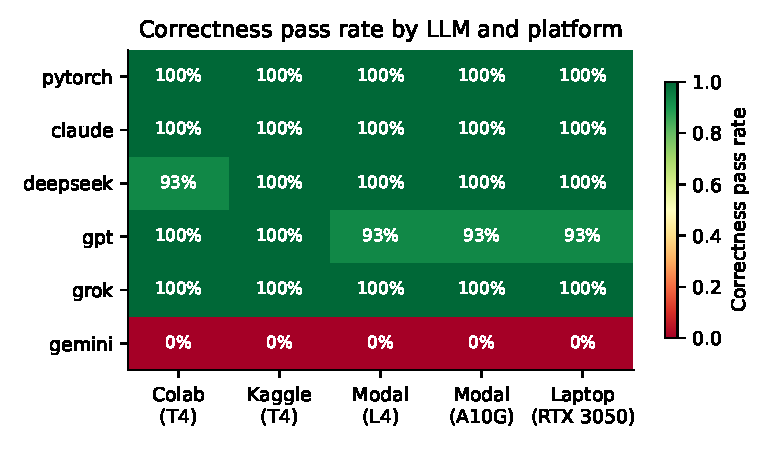
\includegraphics[width=0.48\textwidth]{figures/fig1_correctness_matrix.pdf}
\caption{Correctness pass rate by LLM and execution platform.}
\label{fig:correctness}
\end{figure}

\subsection{Performance Comparison}

Fig.~\ref{fig:latency} compares mean execution time for a representative compute-bound kernel
(matmul, largest tested size) and a representative memory-bound kernel (reduction, largest tested
size) across the four GPUs, for every LLM whose kernel passed correctness. Two findings stand out.
First, the PyTorch baseline is 5--25$\times$ faster than every LLM-generated kernel on every
GPU for the compute-bound kernels, reflecting the maturity of cuDNN/cuBLAS relative to a single-
shot LLM-generated implementation. Second, for matmul specifically, all four working LLMs
(Claude, DeepSeek, GPT, Grok) perform nearly identically on every GPU (within a few percent of each
other), since all four converged on a similar shared-memory tiling strategy; the LLMs
differentiate far more sharply on attention, discussed next.

\begin{figure}[htbp]
\centering
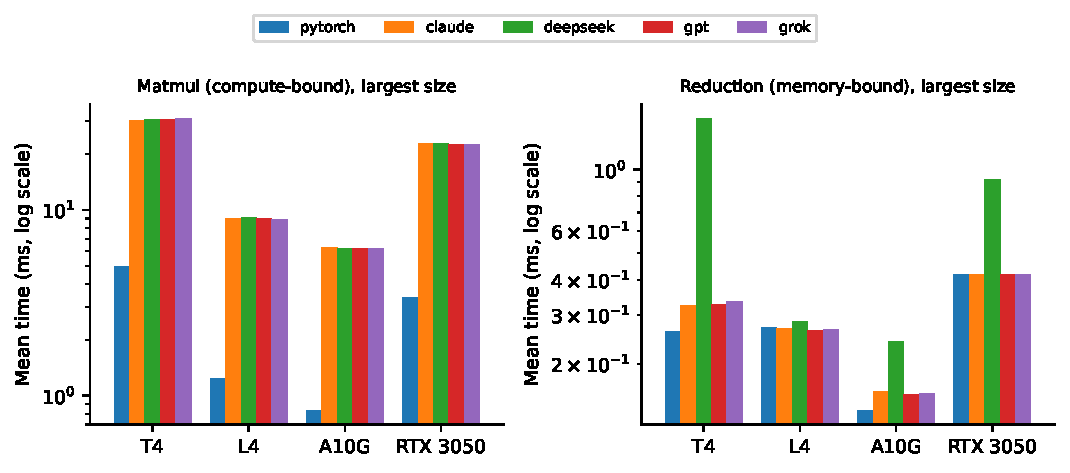
\includegraphics[width=0.5\textwidth]{figures/fig2_latency_comparison.pdf}
\caption{Mean latency (log scale) for matmul (compute-bound) and reduction (memory-bound) at the
largest tested size, by GPU and source.}
\label{fig:latency}
\end{figure}

Attention is the kernel where implementation strategy, not just raw hardware, determines
performance. DeepSeek's attention kernel implements genuine online-softmax (``flash-attention
style'') accumulation, never materializing the full sequence-length-squared attention matrix in
global memory, while Claude's and GPT's kept a full per-query-row score buffer in shared memory,
and Grok's materializes the complete attention matrix in global memory. The resulting mean
latencies at the largest tested size (seq\_len 2048) were, in milliseconds: on the Tesla T4,
DeepSeek 40.6 versus Claude 61.8, GPT 64.5, and Grok 65.8; on the NVIDIA L4, DeepSeek 17.7 versus
21.6, 26.1, and 19.1 respectively; on the A10G, DeepSeek 14.2 versus 14.4, 19.5, and 14.7; and on
the RTX 3050, DeepSeek 43.4 versus 49.0, 67.7, and 50.8. DeepSeek's attention kernel is therefore
the fastest LLM-generated implementation on every single GPU tested, by margins of 13--44\%,
directly attributable to its superior algorithmic choice rather than to GPU-specific tuning.

Fig.~\ref{fig:roofline} shows every passing (kernel, LLM, GPU) measurement plotted against each
GPU's theoretical roofline ceiling. All measured points fall well below their GPU's ceiling,
confirming that none of the hand/LLM-written kernels approach peak achievable throughput -- expected,
since none implement GPU-generation-specific optimizations such as double buffering or tensor-core
paths, unlike the heavily-tuned PyTorch/cuDNN baseline.

\begin{figure}[htbp]
\centering
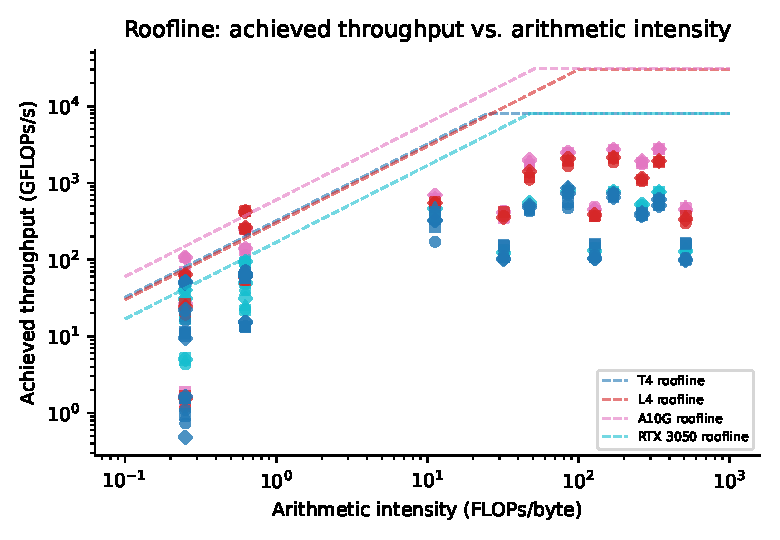
\includegraphics[width=0.48\textwidth]{figures/fig3_roofline.pdf}
\caption{Achieved throughput vs.\ arithmetic intensity for every passing measurement, with each
GPU's analytical roofline ceiling overlaid (dashed).}
\label{fig:roofline}
\end{figure}

\subsection{Power Efficiency}

Fig.~\ref{fig:power} reports GFLOPs per watt, pooling all four GPUs, for the three compute-bound
kernels. The PyTorch baseline is 10--50$\times$ more power-efficient than any LLM-generated kernel,
widening further for attention (123.9 GFLOPs/W for PyTorch versus 2.5--4.0 for the four working
LLMs) than for matmul (311.5 versus 12.9--32.6), indicating that the efficiency gap between
hand-optimized and LLM-generated code grows with kernel complexity rather than staying constant.

\begin{figure}[htbp]
\centering
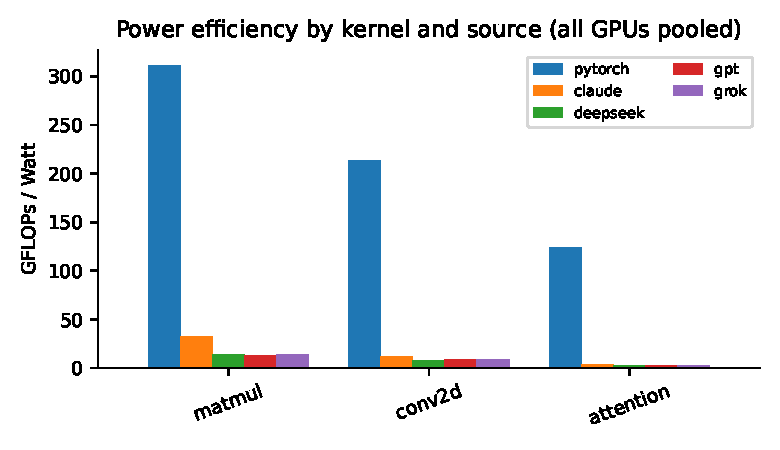
\includegraphics[width=0.48\textwidth]{figures/fig4_power_efficiency.pdf}
\caption{Power efficiency (GFLOPs/Watt) by kernel type and source, pooled across all four GPUs.}
\label{fig:power}
\end{figure}

\subsection{Run-to-Run Variance on Shared Cloud GPUs}

To assess whether a single benchmark run on a free-tier cloud GPU is representative, we pushed an
independent second execution of the full sweep to Kaggle, using the identical code and GPU model
(Tesla T4), several hours after the first. Matching 74 (kernel, LLM, size) cells across both runs,
the mean timing difference was $-4.1\%$ (second run faster on average) with a standard deviation
of $11.2\%$ and a range of $-38.8\%$ to $+43.8\%$. Critically, the largest deviations were not
random: matmul at the largest tested size (2048$\times$2048$\times$2048) was consistently
18--21\% faster in the second run across all four working LLMs simultaneously (Claude $-18.0\%$,
DeepSeek $-19.3\%$, GPT $-20.4\%$, Grok $-20.9\%$), indicating a systematic difference in the
underlying hardware or tenancy state between sessions rather than per-kernel noise. We also
observed one correctness outcome flip between the two runs -- DeepSeek's reduction kernel at its
largest input size passed in the first run and failed in the second, on identical hardware and
code, confirming that this specific failure mode (Section~\ref{sec:discussion}) is a genuine
run-to-run numerical non-determinism rather than a platform-specific trait.

\subsection{Sustained-Load Thermal Behavior}

We ran a dedicated ten-minute sustained-load sweep on the RTX 3050 laptop GPU, repeatedly invoking
Claude's attention kernel at the largest tested size and sampling GPU temperature, clock speed, and
power draw every five seconds (Fig.~\ref{fig:thermal}). GPU temperature rose from 51\,$^{\circ}$C
to 74\,$^{\circ}$C over the ten minutes while power draw remained essentially flat at
$79.8 \pm 0.07$\,W throughout -- that is, the GPU was power-limited by its 80\,W configuration for
the entire run, not thermal-limited. Clock speed drifted down modestly from 1927\,MHz to
1897\,MHz ($-1.6\%$) once temperature exceeded approximately 70\,$^{\circ}$C, and mean per-call
latency correspondingly rose from 129.6\,ms (early in the run) to 133.0\,ms (at the end), a
$2.6\%$ slowdown. This is a mild, real secondary thermal throttle layered on top of a power
ceiling that binds from the very first measurement -- a qualitatively different and more benign
behavior than a thermal cliff, and one that would not be visible from any of our other GPUs, since
none of the three datacenter GPUs in this study are power- or thermal-constrained in the same way a
laptop chassis is.

\begin{figure}[htbp]
\centering
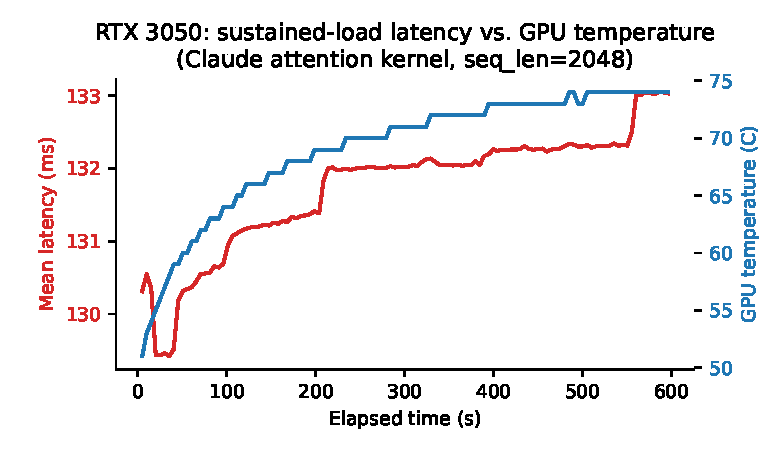
\includegraphics[width=0.48\textwidth]{figures/fig6_thermal_sweep.pdf}
\caption{RTX 3050 sustained-load latency and GPU temperature over a ten-minute window.}
\label{fig:thermal}
\end{figure}

\section{Predictive Performance Model}

\subsection{Roofline-Based Analytical Prediction}

For a given (kernel, input size, GPU), we predict execution time analytically as
$t_{\text{pred}} = \max(\text{FLOPs}/P_{\text{compute}}, \text{Bytes}/P_{\text{bandwidth}})$,
where FLOPs and Bytes are computed directly from the kernel's known access pattern and
$P_{\text{compute}}$, $P_{\text{bandwidth}}$ are the target GPU's peak FP32 throughput and memory
bandwidth from its specification sheet (Table~\ref{tab:gpus}). This equation requires no
measurement of the target GPU whatsoever. Evaluated against all passing measurements, its
mean absolute error (MAE) is 14.76\,ms for the T4, 4.89\,ms for the L4, 3.41\,ms for the A10G, and
11.68\,ms for the RTX 3050 -- already a reasonable first-order estimate, though one that
necessarily cannot capture the gap between a naive/LLM-written kernel's achieved occupancy and
the idealized peak the roofline model assumes.

\paragraph{A critical measurement caveat: TF32.} Ampere-and-newer GPUs (L4, A10G, RTX 3050) enable
TensorFloat-32 by default in cuDNN/cuBLAS, silently reducing the PyTorch reference
implementation's effective precision relative to the hand-written FP32 CUDA kernels it is compared
against; Turing (T4) has no TF32 path and is therefore unaffected. Before we explicitly disabled
TF32 (\texttt{torch.backends.cudnn.allow\_tf32 = False},
\texttt{torch.backends.cuda.matmul.allow\_tf32 = False}) in our harness, several conv2d and
attention correctness checks failed spuriously on the L4 with errors (0.02--0.048) just over our
tolerance threshold -- not because the generated kernels were wrong, but because the reference
they were being checked against was computing a different, lower-precision result. This is an
easy trap for any cross-architecture GPU benchmark that compares a PyTorch reference against
hand-written FP32 code, and to our knowledge is rarely called out explicitly in the LLM-generated-
kernel evaluation literature.

\subsection{Hybrid Residual Correction and Leave-One-GPU-Out Validation}

We additionally fit a residual-correction model: for every measured row, we compute
$r = t_{\text{actual}} - t_{\text{pred}}$ and train a regressor (linear regression or random
forest, both from scikit-learn) to predict $r$ from the target GPU's specification-sheet features
(SM count, clock, bandwidth, FP32/FP16 throughput, L2 cache, TDP) plus the kernel's arithmetic
intensity. The final hybrid prediction for an unmeasured GPU is
$t_{\text{hybrid}} = t_{\text{pred}} + \hat{r}$. We validate this honestly via leave-one-GPU-out
cross-validation: the correction model is trained on three GPUs and evaluated, without any of its
own data, on the fourth.

\begin{table}[htbp]
\caption{Leave-One-GPU-Out Mean Absolute Error (ms)}
\label{tab:logocv}
\centering
\begin{tabular}{@{}lccc@{}}
\toprule
Held-out GPU & Roofline only & Hybrid (linear) & Hybrid (RF) \\
\midrule
Tesla T4 & 14.76 & 12.23 (+17.2\%) & 9.25 (\textbf{+37.3\%}) \\
NVIDIA L4 & 4.89 & 11.82 ($-$141.6\%) & 4.53 (+7.3\%) \\
NVIDIA A10G & 3.41 & 12.05 ($-$253.4\%) & 6.38 ($-$87.1\%) \\
RTX 3050 Laptop & 11.68 & 10.75 (+8.0\%) & 5.05 (\textbf{+56.8\%}) \\
\bottomrule
\end{tabular}
\end{table}

Table~\ref{tab:logocv} and Fig.~\ref{fig:logocv} summarize the result. The random-forest
correction improves on the roofline-only baseline for three of four held-out GPUs, substantially
so for the T4 and the RTX 3050 (+37.3\% and +56.8\% MAE reduction respectively), but makes the
A10G prediction markedly worse ($-87.1\%$). The linear-regression correction is unreliable in
general, improving only the T4 and RTX 3050 cases modestly while badly overcorrecting for both the
L4 and A10G. We interpret this as direct evidence that four GPUs, spanning three architecture
generations, is on the edge of what is needed for this kind of correction term to begin
generalizing (the random forest result is a measurable improvement over having only two GPUs, which
we verified overcorrected in every single held-out case in an earlier iteration of this analysis),
but is not yet enough to guarantee the correction helps rather than hurts for an arbitrary new
GPU. We report this as an honest limitation rather than present the improving cases alone.

\begin{figure}[htbp]
\centering
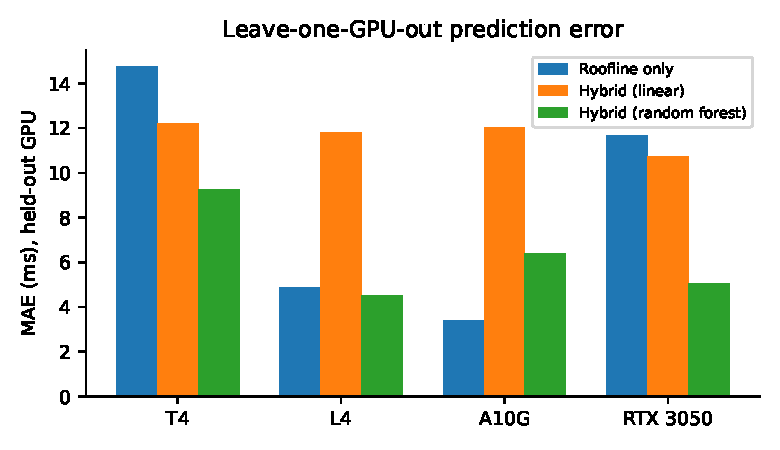
\includegraphics[width=0.48\textwidth]{figures/fig5_logo_cv.pdf}
\caption{Leave-one-GPU-out prediction error: analytical roofline alone versus hybrid correction
(linear and random forest).}
\label{fig:logocv}
\end{figure}

\section{Discussion: Reproducible LLM Kernel Defects}
\label{sec:discussion}

Three defects recur across our results with enough consistency to characterize precisely rather
than dismiss as noise.

\textit{Gemini: systematic compilation failure.} Every one of Gemini's 25 generated kernels
(five kernel types, implicitly re-triggered on every platform) fails to compile, with an identical
root cause each time: the generated CUDA source calls
\texttt{at::cuda::getCurrentCUDAStream()} and \texttt{C10\_CUDA\_KERNEL\_LAUNCH\_CHECK()} without
including the headers (\texttt{<ATen/cuda/CUDAContext.h>}, \texttt{<c10/cuda/CUDAException.h>})
that declare them. This is a simple, mechanically fixable omission, but its perfect consistency
across five independent kernel-generation prompts indicates a systematic gap in this model's
training data or prompting for this specific PyTorch C++ extension pattern, not an isolated
mistake.

\textit{GPT: architecture-dependent correctness bug.} GPT's attention kernel fails its
correctness check at the smallest tested input shape (batch 8, heads 8, seq\_len 128, head\_dim
64) on every Ampere/Ada GPU we tested (L4, A10G, RTX 3050 Laptop) and passes on the Turing T4,
reproduced independently three times on three separate GPUs. Because the same compiled binary
behaves differently depending on compute capability, this points to a warp-scheduling or
shared-memory race condition that happens to be masked by Turing's scheduling behavior but exposed
on newer architectures -- a class of bug that would be easy to miss if a developer validated an
LLM-generated kernel on only one GPU generation. This contrasts with Sarkar's
cross-hardware result~\cite{correctness-illusion}, in which seeded, hardware-independent bugs
produced identical pass/fail verdicts across five GPU classes; our finding is that the underlying
numerical behavior itself, not just a verification oracle's verdict on it, can diverge by
architecture.

\textit{DeepSeek: borderline numerical non-determinism.} DeepSeek's reduction kernel, which
accumulates partial sums via \texttt{atomicAdd}, fails its correctness check at its largest tested
input size (16{,}777{,}216 elements) intermittently: it failed on Colab's T4, passed on Kaggle's
first T4 run, failed on Kaggle's second (independent, same-hardware) T4 run, and passed on the
L4, A10G, and RTX 3050. This pattern -- inconsistent even across identical hardware and code -- is
best characterized as the kernel's accumulation order being close enough to our numerical
tolerance threshold that ordinary thread-scheduling nondeterminism between runs decides the
outcome, rather than as a platform-specific or purely deterministic bug.

\section{Threats to Validity and Limitations}
\label{sec:limitations}

Our study has five limitations we consider important to state plainly rather than understate.
First, each (LLM, kernel) pair was generated exactly once; we cannot distinguish a model that
reliably produces a given defect from one that produced it on an unlucky single sample, and
repeated sampling would be the highest-leverage addition to strengthen the comparative-LLM
findings in Section~\ref{sec:discussion}. Second, kernels were generated via each provider's chat
interface rather than its API, so sampling temperature was not controlled or recorded, precluding
any analysis of generation-parameter sensitivity. Third, only three input sizes were tested per
kernel, enough to establish the direction of a GPU-to-GPU or LLM-to-LLM comparison but not to fit
a precise scaling curve. Fourth, and most importantly for Section~\ref{sec:results-correctness}'s
predictive model, four GPUs is a small sample for a regression intended to generalize to arbitrary
unmeasured hardware; Table~\ref{tab:logocv}'s A10G result is direct evidence of this limit rather
than a transient bug, and we would not recommend deploying the hybrid correction model as-is
without validating on additional, architecturally distinct GPUs first. Fifth, the speedup and
power-efficiency ratios we report (Sections~\ref{sec:results}-B and -C) are computed against a
single PyTorch baseline per operation at a single implementation each; KernelBench-Verified's
audit~\cite{kernelbench-verified} shows that apparent LLM-kernel speedups in this style of
comparison can be inflated by a weak or non-representative baseline, so our absolute speedup
numbers should be read as relative to \emph{this particular} PyTorch implementation and configuration
rather than as a definitive ceiling on what either side could achieve.

\section{Conclusion and Future Work}

We presented a correctness-gated, multi-platform, multi-architecture benchmarking framework for
LLM-generated CUDA kernels and used it to identify three reproducible defect patterns -- one
systematic, one architecture-dependent, one run-to-run non-deterministic -- that a single-GPU
evaluation would not reliably distinguish from each other. We further showed that a widely-used
GPU numerical default (TF32) can silently invalidate a cross-architecture correctness comparison
unless explicitly controlled for, and that a hybrid roofline-plus-regression performance predictor
is only partially reliable at $n=4$ training GPUs, improving prediction for three of four held-out
cases but meaningfully degrading it for the fourth. Future work should prioritize, in order of
expected impact: benchmarking additional architecturally distinct GPUs to test whether the hybrid
correction's reliability continues to improve with more training points; repeated sampling of each
(LLM, kernel) pair to convert the single-sample defect observations in
Section~\ref{sec:discussion} into statistically characterized failure rates; and controlled
generation-temperature sweeps via each provider's API to test whether the observed defects are
sensitive to sampling temperature. Hardware-performance-counter profiling, as used for GPU kernel
characterization and autotuning in~\cite{hwcounters1,hwcounters2}, could additionally help isolate
the root cause of GPT's architecture-dependent bug (Section~\ref{sec:discussion}) by directly
comparing warp-execution and memory-access counters between the passing (Turing) and failing
(Ampere/Ada) runs, rather than inferring the mechanism from behavior alone as we do here.

\begin{thebibliography}{00}

\bibitem{roofline} S. Williams, A. Waterman, and D. Patterson, ``Roofline: An insightful visual
performance model for multicore architectures,'' \textit{Communications of the ACM}, vol. 52,
no. 4, 2009, doi: 10.1145/1498765.1498785.

\bibitem{kernelbench} A. Ouyang, S. Guo, S. Arora, A. L. Zhang, W. Hu, C. Ré, and A. Mirhoseini,
``KernelBench: Can LLMs write efficient GPU kernels?,'' in \textit{Proc. 42nd Int. Conf. Machine
Learning (ICML)}, 2025. [Online]. Available: arXiv:2502.10517.

\bibitem{turing} NVIDIA Corporation, ``NVIDIA Turing GPU Architecture Whitepaper,'' 2018.

\bibitem{ampere} NVIDIA Corporation, ``NVIDIA Ampere GA102 GPU Architecture Whitepaper,'' 2020.

\bibitem{ada} NVIDIA Corporation, ``NVIDIA Ada GPU Architecture Whitepaper,'' 2022.

\bibitem{cudabench} J. Zhu \textit{et al.}, ``CUDABench: Benchmarking LLMs for Text-to-CUDA
Generation,'' 2026. [Online]. Available: arXiv:2603.02236.

\bibitem{correctness-illusion} D. Sarkar, ``The Correctness Illusion in LLM-Generated GPU
Kernels,'' 2026. [Online]. Available: arXiv:2606.20128.

\bibitem{kernelbenchx} H. Wang \textit{et al.}, ``KernelBench-X: A Comprehensive Benchmark for
Evaluating LLM-Generated GPU Kernels,'' 2026. [Online]. Available: arXiv:2605.04956.

\bibitem{kernelbench-verified} Zhang \textit{et al.}, ``KernelBench-Verified: Do LLM-Generated
Kernels Actually Beat PyTorch?,'' 2026. [Online]. Available: arXiv:2607.16241.

\bibitem{hwcounters1} M. Zigon and S. Song, ``Characterizing GPU Kernel Behavior via Hardware
Performance Counters and Machine Learning,'' in \textit{Proc. Int. Conf. Computational Science
(ICCS)}, 2020.

\bibitem{hwcounters2} J. Filipovi\v{c}, J. Hozzov\'{a}, A. Nezarat, J. O\v{l}ha, and F. Petrovi\v{c},
``Using hardware performance counters to speed up autotuning convergence on GPUs,''
\textit{J. Parallel Distrib. Comput.}, 2022. [Online]. Available: arXiv:2102.05297.

\end{thebibliography}

\end{document}
